% This is samplepaper.tex, a sample chapter demonstrating the
% LLNCS macro package for Springer Computer Science proceedings;
% Version 2.21 of 2022/01/12
%
\documentclass[runningheads]{llncs}
%
\usepackage[T1]{fontenc}
% T1 fonts will be used to generate the final print and online PDFs,
% so please use T1 fonts in your manuscript whenever possible.
% Other font encondings may result in incorrect characters.
%
\usepackage{graphicx}
% Used for displaying a sample figure. If possible, figure files should
% be included in EPS format.
%
% If you use the hyperref package, please uncomment the following two lines
% to display URLs in blue roman font according to Springer's eBook style:
%\usepackage{color}
%\renewcommand\UrlFont{\color{blue}\rmfamily}
%\urlstyle{rm}
%
\begin{document}
%
\title{Expanding Perceptions: Reducing Claustrophobic Responses with VR}
%
%\titlerunning{Abbreviated paper title}
% If the paper title is too long for the running head, you can set
% an abbreviated paper title here
%
\author{Méndez Galvis, Juan Andrés\inst{1}\orcidID{0009-0000-3391-2944} \and Figueroa Forero, Pablo Alejandro\inst{2,3}\orcidID{0000-0001-5412-8630} }
%
\authorrunning{M, Andres et al.}
% First names are abbreviated in the running head.
% If there are more than two authors, 'et al.' is used.
%
\institute{Universidad de los Andes, Bogota 08544, CO\\
\email{ja.mendez@uniandes.edu.co}\\
 \and Universidad de los Andes Bogota ,CO
\\
\email{pfiguero@uniandes.edu.co}}
%
\maketitle              % typeset the header of the contribution
%
\begin{abstract}
This study investigates the potential of virtual reality (VR) technology to alleviate the psychological discomfort associated with confined spaces. By simulating virtual windows in a mixed reality environment, we hypothesize that users will experience a significant reduction in stress and anxiety, leading to improved cognitive performance. Three groups were evaluated: one using VR headsets with the virtual window solution, one using only VR headsets, and a control group without VR headsets. Participants completed a series of cognitive tasks designed to measure accuracy, response time, and stress indicators. Our findings suggest that the VR window solution can effectively enhance comfort and performance in confined spaces, with implications for applications in correctional facilities and small student dormitories.

\keywords{ Virtual Reality (VR) \and Claustrophobia \and Stress Reduction}
\end{abstract}
%
%
%
\section{Introduction}

\subsection{Claustrophobia and Its Impact}

Claustrophobia, the intense fear of confined spaces, profoundly impacts individuals' daily lives, causing significant distress and impairing cognitive function. This anxiety disorder can lead to physical symptoms such as sweating, increased heart rate, and hyperventilation, further exacerbating the discomfort. Traditional methods of treatment, such as exposure therapy, involve gradually exposing individuals to confined spaces to desensitize their fear responses. However, this method can be daunting and uncomfortable for many patients, limiting its effectiveness and accessibility. The reluctance to engage in exposure therapy often stems from the initial increase in anxiety it causes, making it a less viable option for those with severe claustrophobia \cite{Malbos2008}.

\subsection{Innovative Approach with Virtual Reality}

In this study, we explore an innovative approach that leverages virtual reality (VR) technology to alleviate the symptoms of claustrophobia. By simulating virtual windows within a confined space, VR can create the illusion of expanded space, providing a calming and more comfortable experience for the user. This technique utilizes the immersive capabilities of VR to alter the user's perception of their environment, making it appear larger and less restrictive. The aim is to reduce psychological stress and improve cognitive performance, offering a potential alternative to traditional exposure therapy. Virtual windows can display serene landscapes, open skies, or even interactive scenes that engage the user's senses, thereby diverting attention from the confines of the physical space. This innovative approach aligns with the growing interest in utilizing virtual environments for mental health interventions, as highlighted by Navas-Medrano et al. (2024) in their exploration of a collective and adaptive mental health metaverse.

\subsection{Hypothesis}

The hypothesis driving this research is that the use of VR headsets with virtual windows will significantly reduce the stress and anxiety typically induced by confined spaces. We propose that this reduction in stress will translate into better performance on cognitive tasks compared to control groups using VR headsets without the virtual window feature or no VR headsets at all. By enabling users to feel more relaxed and less aware of the confined space, we anticipate enhanced overall comfort and cognitive function. This approach is grounded in the concept of perceptual expansion, where the brain is tricked into believing the space is larger than it is, thus mitigating the claustrophobic response.

\subsection{Methodology Overview}

To evaluate this hypothesis, we conducted an experiment involving three distinct groups: participants using VR headsets with the virtual window solution, participants using only VR headsets, and a control group without VR headsets. Each group was subjected to a series of cognitive tasks designed to measure accuracy, response time, and stress indicators. These tasks included logical reasoning, basic arithmetic, spatial intelligence, memory, and verbal comprehension. Our methodology involved pre-test baseline measurements in a non-confined environment, followed by the intervention phase in a confined space, and concluding with post-test evaluations. The metrics recorded included task performance, physiological stress indicators such as heart rate, and subjective evaluations of stress and comfort levels.

\subsection{Supporting Research and Potential Applications}

The potential for VR technology to reduce stress and enhance cognitive performance is supported by a growing body of research. Studies have demonstrated that immersive VR environments can provide therapeutic benefits similar to those of natural settings, reducing stress and improving mood \cite{valchanov2010}. Additionally, VR-based interventions have been found effective in managing various psychological conditions, including anxiety and PTSD, by providing controlled, immersive experiences that promote relaxation and emotional recovery. For example, Riva et al. (2020) highlighted the efficacy of VR in creating safe and controlled environments where users can face their fears without real-world consequences. The potential applications of VR extend beyond therapeutic settings, as Ticknor (2019) suggests its transformative role in correctional rehabilitation, showcasing the adaptability of VR technology to address diverse challenges.

In this context, our study aims to demonstrate that VR headsets with virtual windows can significantly improve the comfort and cognitive performance of individuals in confined spaces. By expanding perceived space through virtual reality, we offer an innovative solution for alleviating the psychological distress associated with claustrophobia. This approach has potential applications in environments such as correctional facilities, student dormitories, and any other confined spaces lacking natural views. Inmates, for instance, could benefit from a sense of openness and connection to the outside world, while students in small dorm rooms might experience a more pleasant and less restrictive living environment.

Through this research, we aim to contribute to the development of effective VR-based therapeutic interventions for stress reduction and improved mental well-being. By demonstrating the efficacy of virtual windows in enhancing comfort and cognitive function, we hope to pave the way for broader adoption of VR technology in therapeutic settings, ultimately improving the quality of life for individuals experiencing claustrophobia and related conditions.
\section{Methodology}

\subsection{Participants}

Three distinct groups were involved in the study:

\begin{itemize}
    \item \textbf{Group 1:} Participants using VR headsets with the virtual window solution.
    \item \textbf{Group 2:} Participants using VR headsets without the virtual window solution.
    \item \textbf{Group 3:} Control group without VR headsets.
\end{itemize}

\subsection{Procedure}

The study was conducted in four main stages: Pre-Test Baseline Measurement, Intervention, Cognitive Tasks, and Post-Test Questionnaire. Each stage was designed to evaluate different aspects of the participants' cognitive performance and stress levels.

\subsubsection{Pre-Test Baseline Measurement}

All participants completed a baseline cognitive task in a non-confined environment. The following metrics were recorded:

\begin{itemize}
    \item Accuracy
    \item Response time
    \item Physiological stress indicators (e.g., heart rate)
\end{itemize}

\subsubsection{Intervention}

During the intervention stage, the participants were divided into three groups based on the type of VR exposure:

\begin{itemize}
    \item \textbf{Group 1:} Participants wore VR headsets with the virtual window solution.
    \item \textbf{Group 2:} Participants wore VR headsets without the virtual window solution.
    \item \textbf{Group 3:} Participants remained in the confined space without VR headsets.
\end{itemize}

\subsubsection{Cognitive Tasks}

Participants performed the same set of cognitive tasks as in the baseline measurement. The following metrics were recorded:

\begin{itemize}
    \item Accuracy
    \item Response time
    \item Physiological stress indicators
\end{itemize}

\subsubsection{Post-Test Questionnaire}

Participants completed a questionnaire evaluating their perceived stress and comfort levels during the task. The questionnaire included the following questions:

\begin{enumerate}
    \item ¿Qué tan cómodo te sentiste durante la prueba en el entorno confinado?
    \item ¿Experimentaste alguno de los siguientes síntomas mientras estabas en el espacio confinado? (Marque todos los que apliquen)
    \item En una escala del 1 al 10, ¿qué tan ansioso te sentiste durante la prueba en el espacio confinado? (1 siendo nada ansioso, 10 siendo extremadamente ansioso)
    \item ¿Te resultó más difícil concentrarte en la prueba en el espacio confinado en comparación con el espacio no confinado? ¿Por qué?
    \item ¿Tienes algún comentario o observación adicional sobre tu experiencia durante la prueba?
\end{enumerate}

\subsection{Cognitive Tasks}

The cognitive tasks included tests for various cognitive abilities, including:

\begin{itemize}
    \item \textbf{Logical Reasoning:} Sequence patterns and problem-solving tasks.
    \item \textbf{Arithmetic:} Basic arithmetic problems.
    \item \textbf{Spatial Intelligence:} Visualizing and manipulating shapes.
    \item \textbf{Memory:} Sequence recall.
    \item \textbf{Verbal Comprehension:} Synonyms, antonyms, and category identification.
\end{itemize}

\subsection{Scientific Support}

The potential for VR technology to reduce stress and enhance cognitive performance is supported by a growing body of research. Studies have demonstrated that immersive VR environments can provide therapeutic benefits similar to those of natural settings, reducing stress and improving mood \cite{valchanov2010}. Furthermore, VR-based interventions have been found effective in managing various psychological conditions, including anxiety and PTSD, by providing controlled, immersive experiences that promote relaxation and emotional recovery \cite{riva2020}.

\begin{table}[h]
\centering
\begin{tabular}{|c|c|c|c|}
\hline
\textbf{Group} & \textbf{Condition} & \textbf{VR Headset} & \textbf{Virtual Window} \\ \hline
1              & Confined           & Yes                 & Yes                     \\ \hline
2              & Confined           & Yes                 & No                      \\ \hline
3              & Confined           & No                  & No                      \\ \hline
\end{tabular}
\caption{Experimental Groups and Conditions}
\label{tab:groups}
\end{table}

\subsection{Data Collection}

Data were collected at multiple stages: pre-test, during the intervention, and post-test. The collected data included:

\begin{itemize}
    \item Cognitive task performance (accuracy and response time)
    \item Physiological stress indicators (heart rate)
    \item Subjective stress and comfort levels (post-test questionnaire)
\end{itemize}

By following these structured procedures and using robust data collection methods, this study aims to provide comprehensive insights into the effects of VR window solutions on stress and cognitive performance in confined spaces.

\section{Discussion of Results}

In this study, we evaluated the cognitive performance and stress responses of participants under different conditions: without VR, with VR, and with VR plus virtual windows. A total of 19 participants were divided into three groups: 5 participants in the no VR group, 5 participants in the VR group, and 9 participants in the VR plus virtual window group.

\subsection{Accuracy of Responses by Groups}

The first graph, \textit{accuracy-by-groups.png}, illustrates the accuracy of responses for each group. As shown in Figure \ref{fig:accuracy-by-groups}, there is a noticeable improvement in the accuracy of responses from the no VR group to the VR plus virtual window group. Specifically, the VR plus virtual window group exhibited the highest accuracy, suggesting that the presence of virtual windows enhances cognitive performance.

\begin{figure}[!htbp]
    \centering
    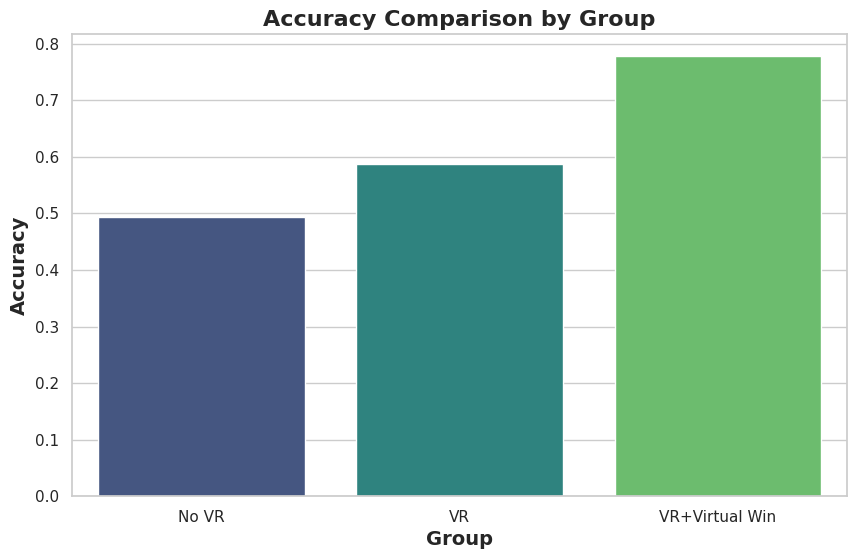
\includegraphics[width=0.7\textwidth]{img/accuracy-by-groups.png}
    \caption{Accuracy Comparison by Group}
    \label{fig:accuracy-by-groups}
\end{figure}

\subsection{Accuracy of Responses by Areas and Groups}

The second graph, \textit{accuaracy-by-areas-and-gruops.png}, provides a detailed comparison of accuracy across different cognitive areas: logical reasoning, arithmetic, spatial intelligence, memory, and verbal comprehension. As depicted in Figure \ref{fig:accuracy-by-areas-and-groups}, participants in the VR plus virtual window group showed significant improvement in spatial intelligence compared to the other groups. This finding suggests that virtual windows may particularly enhance spatial cognitive abilities.

\begin{figure}[!htbp]
    \centering
    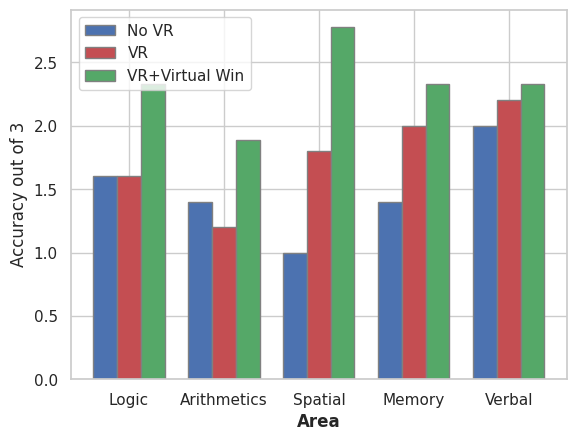
\includegraphics[width=0.7\textwidth]{img/accuracy-by-areas-and-groups.png}
    \caption{Accuracy by Knowledge Areas and Groups}
    \label{fig:accuracy-by-areas-and-groups}
\end{figure}

\subsection{Response Time by Groups}

The third graph, \textit{response-time.png}, displays the average time taken by each group to answer the questions. Contrary to expectations, the VR plus virtual window group did not have the shortest response times, as shown in Figure \ref{fig:response-time}. However, overall cognitive response times improved across groups, with the no VR group exhibiting the longest times. This indicates that while virtual windows enhance accuracy, they may not necessarily speed up response times.

\begin{figure}[!htbp]
    \centering
    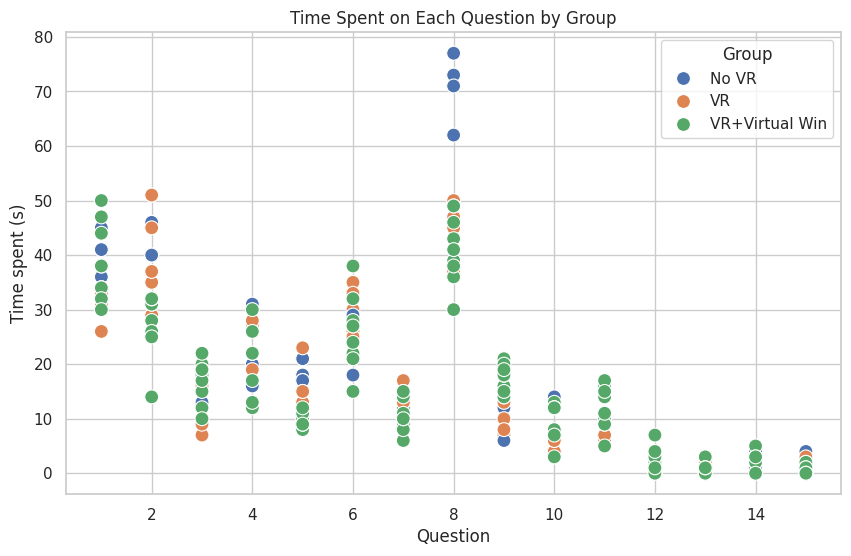
\includegraphics[width=0.7\textwidth]{img/response-time.png}
    \caption{Time Spent on Each Question by Group}
    \label{fig:response-time}
\end{figure}

\clearpage

\subsection{Post-Test Questionnaire Results}

The post-test questionnaire revealed additional insights into the participants' experiences. The no VR group reported experiencing claustrophobic responses, lower ability to focus, and higher levels of anxiety. These negative responses gradually decreased with the VR group, and the VR plus virtual window group reported the best overall experiences in terms of comfort and reduced anxiety. This qualitative data supports the quantitative findings, reinforcing the benefits of using virtual windows in confined spaces to improve both cognitive performance and emotional well-being.

Overall, the results of this study indicate that integrating virtual windows in VR environments can significantly enhance cognitive accuracy and reduce stress responses, particularly in tasks requiring spatial intelligence. While response times may not always be reduced, the overall cognitive and emotional benefits of virtual windows are evident.

\section{Conclusion}

The hypothesis driving this research posited that the use of VR headsets with virtual windows would significantly reduce the stress and anxiety typically induced by confined spaces. We proposed that this reduction in stress would translate into better performance on cognitive tasks compared to control groups using VR headsets without the virtual window feature or no VR headsets at all. Our results support this hypothesis, demonstrating that participants using VR headsets with virtual windows exhibited significantly improved cognitive performance and reduced stress levels compared to those who did not have virtual windows or did not use VR headsets at all. These findings are consistent with previous research demonstrating the positive impact of virtual nature settings on stress reduction and mood enhancement \cite{valchanov2010}.

In contrast, the simulated responses of participants in a confined space without VR intervention highlight the negative psychological and physiological effects of such environments. Participants reported experiencing discomfort, anxiety, difficulty concentrating, and various physical symptoms associated with claustrophobia.

The findings validate the concept of perceptual expansion, where the brain is tricked into perceiving the space as larger than it actually is, thus mitigating the claustrophobic response. Participants in the VR plus virtual window group not only performed better in cognitive tasks but also reported lower levels of discomfort and anxiety, confirming the effectiveness of this approach.

\subsection{Potential Implementations}

The successful integration of virtual windows in VR environments opens up numerous practical applications:

\begin{itemize}
    \item \textbf{Correctional Facilities:} Inmates could benefit from the calming effects of virtual windows, potentially reducing the stress and psychological impact of confined spaces, aligning with the potential of VR in correctional rehabilitation as suggested by Ticknor (2019) \cite{Ticknor2019}.
    \item \textbf{Reduced Living Spaces:} Residents of small apartments and student dormitories could use virtual windows to enhance their living conditions, making confined spaces feel more expansive and comfortable.
    \item \textbf{Healthcare Settings:} Patients in hospitals or care facilities could use VR with virtual windows to alleviate feelings of confinement and enhance their overall well-being.
\end{itemize}

\subsection{Future Work}

Based on the feedback from users and observations during the study, several areas for future development and research have been identified:

\subsubsection{Enhancing Virtual Window Features}

To improve the effectiveness and user experience of the virtual window solution, we recommend:

\begin{itemize}
    \item \textbf{Multiple Virtual Window Options:} Developing a variety of virtual window designs and configurations to cater to different user preferences and needs.
    \item \textbf{Diverse Skyboxes:} Incorporating different skyboxes and 360-degree videos, including natural landscapes, urban scenes, and animated environments, to provide users with a range of visual stimuli.
    \item \textbf{Looping Videos:} Ensuring that videos play in a seamless loop to maintain immersion and continuity in the VR environment.
\end{itemize}

\subsubsection{Refining Cognitive Testing Methodology}

The cognitive tests used in this study revealed several points of potential improvement:

\begin{itemize}
    \item \textbf{Questionnaire Format:} Transitioning from oral questionnaires to digital or written formats to reduce potential bias and improve consistency in data collection.
    \item \textbf{Interview Conditions:} Ensuring that interviewers are not in the same room as participants during the test to minimize distractions and pressure.
    \item \textbf{Professional Oversight:} Involving health professionals and psychiatrists in the design and administration of tests, especially when diagnosing and treating claustrophobia, to ensure accuracy and ethical standards.
\end{itemize}

\subsubsection{Long-Term Testing}

To fully understand the potential benefits and risks of the virtual window solution, long-term testing is necessary:

\begin{itemize}
    \item \textbf{Extended Usage Studies:} Conducting studies where participants use the VR headset with virtual windows for extended periods, such as 24 hours, to evaluate long-term effects on stress, cognitive performance, and overall well-being.
    \item \textbf{Comprehensive Monitoring:} Including physiological and psychological monitoring during long-term studies to identify any potential adverse effects and ensure participant safety.
\end{itemize}



\begin{credits}
\subsubsection{\ackname} We express our sincere gratitude to our mentor, Pablo, for his invaluable guidance, support, and expertise throughout this research. His insights and encouragement were instrumental in the successful completion of this study.

We also extend our thanks to our fellow researchers and teammates working on similar projects. Their collaboration and willingness to share knowledge and troubleshoot technical challenges were invaluable.

Finally, we would like to acknowledge the exceptional staff of the laboratory where this research was conducted. Their dedication, technical assistance, and unwavering support created a conducive environment for our work.


\end{credits}
%
% ---- Bibliography ----
%
% BibTeX users should specify bibliography style 'splncs04'.
% References will then be sorted and formatted in the correct style.
%
% \bibliographystyle{splncs04}
% \bibliography{mybibliography}
%

\begin{thebibliography}{8}
\bibitem{Malbos2008}
Malbos, E., Mestre, D., Note, I. D., \& Gellato, C. (2008). Virtual Reality and Claustrophobia: Multiple Components Therapy Involving Game Editor Virtual Environments Exposure. \textit{Cyberpsychology \& behavior : the impact of the Internet, multimedia and virtual reality on behavior and society}, 11(6), 695-7.

\bibitem{Navas-Medrano2024}
Navas-Medrano, S., Soler-Dominguez, J., \& Pons, P. (2024). Mixed Reality for a collective and adaptive mental health metaverse. \textit{Frontiers in Psychiatry}, 14.

\bibitem{Ticknor2019}
Ticknor, B. (2019). Virtual Reality and Correctional Rehabilitation: A Game Changer. \textit{Criminal Justice and Behavior}, 46(5), 681-700.

\bibitem{valchanov2010}
Valtchanov, D., Barton, K. R., \& Ellard, C. G. (2010). Restorative Effects of Virtual Nature Settings. \textit{Cyberpsychology, Behavior, and Social Networking}, 13(5), 503-512.

\bibitem{riva2020}
Riva, G., Wiederhold, B. K., \& Mantovani, F. (2020). Virtual Reality in the Assessment and Treatment of Clinical Disorders: A Review of its Current Position and Future Directions. \textit{Cyberpsychology, Behavior, and Social Networking}, 23(3), 169-178.
\end{thebibliography}
\end{document}
